\chapter{Transfer Learning}\label{transfer-learning}

Con Transfer Learning si intente l'azione di riutilizzare una rete preaddestrata come una \gls{cnn} addestrata con un milione di immagini in mille classi, per altri scopi senza dover riaddestrare la \gls{cnn} riaddrestrare la rete da zero. Senza nessuna azione di riaddestramento della rete la classificazione di una immagine non darà il risultato sperato, quindi almento in parte la rete è da riaddestrare in quanto la rete classicifica per ciò che è stata allenata. Però la struttura di una rete è tale da poter riutilizzare senza problemi. 

\section{Riutilizzo di una \gls{cnn} preaddestrata}\label{riutilizzo-di-una-cnn-preaddestrata}

Per riutilizzare una rete preaddestrata si parte dalla rete e si rimuovono gli ultimi livelli, cioè quelli di classificazione finale e si lasciano quelli di feacture extractor, la rete senza i livelli finali è può essere usata come feacture extractor. Per esempio si può usare una SVM per la classificazione finale, oppure si possono riaggiungere layer dello stesso tipo di quelli originali ovviamente riadattati al numero di classi del programma, a differenza dei layer originali essi hanno i pesi non inizializzati, questa tecnica si chiama fine-tuning. È una tecnica molto usata in quanto il training di \gls{cnn} complesse (es. AlexNet) su dataset di grandi dimensioni (es. ImageNet) può richiedere giorni/settimane di tempo macchina, anche se eseguito su Hardware dedicato. Una volta che la rete è stata addestrata, il tempo richiesto per la classificazione di un  pattern (\gls{propagazione forward} o inference) è in genere inferiore\cite{yosinski_tl}\cite{unibo_maltoni_ml}.

In genere è da sottolineare che addestrare da zero una \gls{cnn} porta a risultati migliori, ma richiede una potenza di calcolo molto più  elevata, oltre che dei dataset molto grandi, per evitare l'\gls{overfitting}. L'addestramento di una \gls{cnn} funziona molto bene su grandi insiemi di dati, tuttavia su piccoli insiemi di dati non riesce a raggiungere guadagni significativi e proprio in questo caso viene utilizzato il transfer learning\cite{joel_tl}.

Il transfer learning è un metodo molto utilizzato nella computer vision, in quanto permette l'uso della conoscenza acquisita per un
compito, come riconoscere le immagini del dataset ImageNet, per risolvere quelli correlati, come riconoscere immagini di un altro dataset, in quanto si basa sul fatto che
funzionalità riguardanti l'estrazione di caratteristiche di basso livello
(per esempio, bordi, forme e angoli) possono essere condivise tra i vari compiti di una rete, nel nostro caso: classificare le immagini in 1000 classi o classificare immagini sfuocate e non sfuocate\cite{patrini_tl}.




\section{Fine-Tuning}\label{fine-tuning}

Nell'approccio fine-tuning del Transfer Learning si parte con una rete pre addestrata su un problema simile e:
\begin{enumerate}
    \item Si rimpiazza il livello di output con un nuovo livello di output \gls{SoftMax} (adeguando il numero di classi) ed altri livelli finali, come i \gls{fully-connected}.
    \item Come valori iniziali dei pesi si utilizzano quelli della rete pre-trained, tranne che per le connessioni tra il penultimo e ultimo livello i cui pesi sono inizializzati random.
    \item Si eseguono nuove iterazioni di addestramento per ottimizzare i pesi rispetto alle peculiarità del nuovo dataset (non è necessario che il dataset sia di grandi dimensioni, ma per migliorare le prestazioni si usa data augmentation e preprocessing).
\end{enumerate}

In generale, tutti i pesi sono pesi allenabili, cioè in  ogni nuovo allenamento essi possono cambiare normalmente attraverso l'algoritmo di ottimizzazione \gls{gd}. In alcuni lavori essi vengono tenuti fissi durante la fase di fine-tuning. L'unico livello integrato che ha pesi non allenabili è il livello di \gls{BatchNormalization}\cite{team_keras_nodate}\cite{lumini_plankton}.

In particolare si possono individuare numerosi approcci per il fine-tuning, tra cui il classico one round:
\paragraph {One round tuning (1R)} \label{one-round-tuning}

È l'approccio standard per il fine-tuning di una reti pre-addestrate: la rete viene inizializzata secondo i pesi pre-addestrati (ottenuti dal dataset ImageNet) e riaddestrata utilizzando il training set del problema target. I pesi degli strati di classificazione vengono azzerrati, i pesi dei primi stati non vengono forzati a rimanere stabili e infine viene usato lo stesso learning rate per tutti gli strati\cite{lumini_plankton}. 

\paragraph{Two rounds tuning (2R)} \label{two-round-tuning}

Questa strategia prevede un primo round di fine-tuning in un dataset simile a quello target e un secondo round utilizzando il training set del problema target. Il primo passo consiste nel fine-tuning della rete, pre-inizializzata secondo i pesi di ImageNet che include immagini di classi non incorporate nel problema target. Il secondo passo è un one round tuning eseguito usando un  dataset esterno. 

L'idea alla base di questo metodo è di insegnare in primo luogo alla rete a riconoscere le laringi, che sono molto diverse dalle immagini nel dataset ImageNet, poi il secondo round viene utilizzato per regolare i pesi di classificazione in base al problema di destinazione. A causa della possibilità di \gls{overfitting}, aumentare il numero di round turning non garantisce un aumento delle prestazioni, soprattuto nel caso di un numero basso di immagini in addestramento\cite{lumini_plankton}. Nella \cref{fig:tl_2rt}  è riportato uno schema dei due metodi, dove ogni colore è relativo a un approccio separato. 

\begin{figure}[ht]
    \centering
    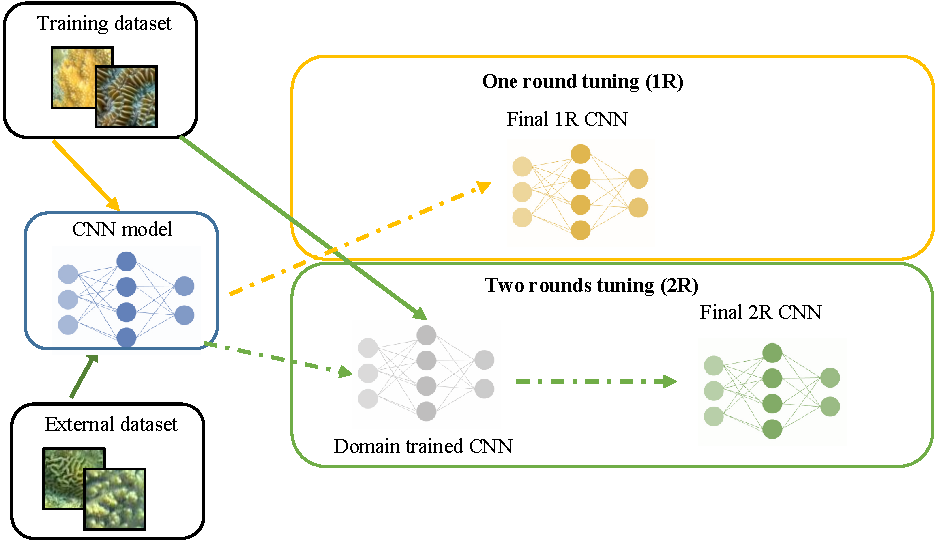
\includegraphics[width=0.7\textwidth]{transfer-learning/tl_2rt.pdf}
    \caption{Uno schema dei due approcci: In giallo il One round turing (1R), in verde il Two round tuning. Le frecce piene denotano l'input per l'addestramento, le frecce tratteggiate denotano i flussi di output (modelli addestrati).}
    \label{fig:tl_2rt}
\end{figure}

In particolare per ottenere buoni risultati con il fine-tuning è importante diminuire la velocità di apprendimento (cioè il fattore learning rate che modifica i pesi), e se necessario congelare alcuni livelli preaddestrati che potrebbero essere alterati senza però.

Se la velocità di apprendimento è troppo alta i risultati peggiorano a casua del gradient descent, in particolare questo può portare a uno stato in cui la rete neurale non riesce a trovare il minimo globale ma solo locale\cite{joel_ft_tl_lfs}\cite{joel_tl}.

\section{Data preprocessing e data augmentation}\label{data-pre-processing-e-augmentation-processing}

La fase di pre-elaborazione è essenziale nelle immagini dei tessuti per rimuovere diversi tipi di rumori, questo vale ancora di più nel caso di transfer learning in quando i dataset di allenamento sono in genere molto inferiori di quello originale oltre che le classi hanno un significato meno generale\cite{joel_tl} in particolare i metodi di preprocessing di immagini sono trattati in \cref{data-preprocessing}.

Inoltre per ottenere prestazioni più elevate nell'accuratezza, la \gls{cnn} richiede grandi insiemi di dati in quanto le performance della \gls{cnn} con piccoli set di dati si deteriora  a causa dell'\gls{overfitting}\cite{joel_tl} in particolare i metodi di data augmentation di immagini sono trattati in \cref{data-augmentation}.





